\chapter{Opis sustava i tehničkih zahtjeva}

\section{Opis problematike hrkanja kao zdravstvenog problema}

Hrkanje je čest poremećaj koji pogađa 20-40\% opće populacije. Ono nastaje kao posljedica vibracije anatomskih struktura u dišnom putu. Treperenje mekog nepca odgovorno je za grubi aspekt zvuka hrkanja. Na hrkanje utječu mnogi faktori kao što su položaj tijela, faza spavanja, dišni putevi i prisutnost ili odsutnost poremećaja disanja tijekom spavanja. Pojava hrkanja može varirati tijekom noći \cite{pevernagie}. 

Iako se hrkanje općenito doživljava kao društvena smetnja, ocjena njegove bučnosti subjektivna je i stoga nedosljedna. Objektivna procjena hrkanja važna je za procjenu učinka terapijskih intervencija. Štoviše, hrkanje nosi informacije koje se odnose na mjesto i stupanj opstrukcije gornjih dišnih putova.

\subsection{Anatomija i klasifikacija hrkanja}
Gornji dišni putovi su područje od nosnica i usana do glasnica. Sastoje se od nosne i usne šupljine, ždrijela i gornjeg dijela grkljana. Ždrijelo je stražnji dio glave i sadrži nekoliko anatomskih orijentira, kao što su meko nepce (velum), nepčani krajnici, korijen jezika i nepčana resica (epiglotis). Epiglotis odvaja ždrijelo od jednjaka i grkljana, koji sadrži glasnice \cite{snoringml}.

\begin{figure}[ht]
	\centering
	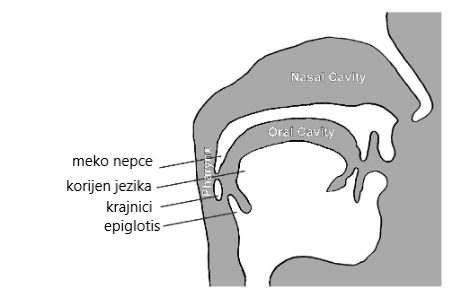
\includegraphics[scale=0.7]{imgs/anatomy}
	\caption{Anatomija gornjih dišnih puteva \cite{snoringml}}
	\label{fig:anatomy}
\end{figure}

Hrkanje je uzrokovano vibracijama struktura mekog tkiva u gornjim dišnim putovima, osobito na fiziološkim suženjima. 
Tijekom sna, tonus mišića se smanjuje, a meko tkivo opušta, povećavajući njegovu sklonost vibriranju. Brzina protoka zraka pri udisaju povećava se u uskim dijelovima gornjih dišnih puteva, izazivajući vibracije tkiva i strujanja zraka, što zauzvrat uzrokuje hrkanje.

Tipična područja koja pridonose stvaranju zvuka hrkanja su meko nepce i njegov vrh, uvula, koja može vibrirati u anteriorno-posteriornom smjeru, nepčani krajnici koji obično vibriraju u lateralnom smjeru, korijen jezika koja može pasti natrag i ograničiti prolaz prema stražnjoj stijenci ždrijela i epiglotis, koji se može spustiti zbog smanjene strukturne krutosti ili zbog stražnjeg pomaka prema stražnjoj stijenci ždrijela.

Za ciljano liječenje hrkanja i srodnih poremećaja disanja povezanih sa spavanjem, ključno je identificirati mehanizme i mjesta koja doprinose sužavanju dišnih puteva i uzrokuju hrkanje ili respiratorne opstrukcije kod pojedinog subjekta.

%\subsection{Klasifikacija hrkanja}

Široko korištena definicija raznih mehanizama hrkanja je VOTE klasifikacija, koja razlikuje četiri razine u kojima se mogu pojaviti hrkanje i sužavanje dišnih puteva:
\begin{itemize}
	\item V - \textit{Velum}: razina mekog nepca, 
	\item O - \textit{Oropharynx}: razina usnog dijela ždrijela,  
	\item T - \textit{Tongue}: razina korijena jezika, 
	\item E - \textit{Epiglottis}: razina epiglotisa. 
\end{itemize}

U radu \cite{bib} uspoređeni su zvukovi hrkanja izazvani tijekom nazendoskopije s onima u prirodnom snu pomoću spektra zvučnih frekvencija. Pacijenti s palatinalnim hrkanjem tijekom nazendoskopije u snu imali su srednju vršnu frekvenciju od 137 Hz. Najveća frekvencija hrkanja u korijenu jezika bila je 1243 Hz, a kombinirano hrkanje nepca i jezika 190 Hz. Središnje frekvencije bile su 371, 1094 i 404 Hz. Epiglotično hrkanje imalo je vršnu frekvenciju od 490 Hz. Iako rezultati pokazuju da inducirano hrkanje sadrži komponentu više frekvencije zvuka koja nije vidljiva tijekom prirodnog hrkanja, korelacija je dovoljno dobra za kategoriziranje zvučnih zapisa hrkanja. 

Također, visina zvuka hrkanja u niskofrekventnom rasponu (<500 Hz) odgovara osnovnoj frekvenciji s pripadajućim harmonicima. Visina hrkanja određena je vibracijom mekog nepca, dok je nepalatalno hrkanje više „nalik buci“ i ima raspršeniju energiju u višim spektralnim podpojasevima (>500 Hz).


\section{Zahtjevi na sustav i opis predloženog rješenja}

Sustav za snimanje pacijenata treba omogućiti snimanje zvuka hrkanja u stvarnim uvjetima. Da bi se to postiglo, potrebno je blizu pacijenta postaviti mikrofon koji snima zvuk i omogućiti bežično slanje snimljenog zvuka u stvarnom vremena na računalo na kojem se zvuk snima. Odabrana je arhitektura gdje se mikrokontrolerski razvojni sustav s mikrofonom koristi za snimanje, a preko svojeg ugrađenog BLE bežičnog sučelja šalje zvuk prema osobnom računalu. 

Prilikom odabira mikrokontrolerskog sustava potrebno je voditi računa da na sebi ima ugrađen i mikrofon i BLE sučelje. Važno je također da sadrži mikrofon prikladan za primanje audio signala iz svih smjerova. Mikrofon također mora moći kvalitetno snimati  zvuk na udaljenosti barem jedan metar od ispitanika, a da bi se provjerilo zadovoljava li se taj uvjet, važno je eksperimentalno provjeriti i analizirati ovisnost udaljenosti mikrofona od izvora zvuka i intenziteta zvučnog zapisa dobivenog snimanjem odabranim hardverom. Na računalu je bilo potrebno razviti aplikaciju koja mora korisniku pružiti jednostavno sučelje za upravljanje snimanjem. Glavna uloga aplikacije je podržati prijem zvučnog zapisa putem BLE sučelja te omogućiti pohranu u datoteku. Također, u sklopu grafičkog korisničkog sučelja potrebno je omogućiti jednostavno uspostavljanje komunikacije s odabranim mikrokontrolerom.

Za potrebe završnog rada odabran je razvojni sustav STM32WB5MM-DK budući da zadovoljava postavljene zahtjeve i ima mogućnost jednostavnog razvoja programske potpore  korištenjem programskim biblioteka proizvođača. Na razvojnom sustav nalazi se mikrokontroler STM32WB5M koji ima ugrađeno BLE komunikacijsko sučelje. Na osobnom računalu korišten je operacijski sustav Linux, iako bi se slično rješenje moglo razviti i na drugim operacijskim sustavima. U radu će biti opisano speficičnosti programske potpore razvijene upravo za Linux kao odabranu platformu rješenja na osobnom računalu. Bežičnim sučeljem prenosi se zvučni signal sniman MEMS mikrofonom s mikrokontrolera na računalo. U okviru programske potpore na osobnom računalu razvijeno je korisničko sučelje za pokretanje komunikacije, prijam i pohranu signala. Blok shema sustava prikazana je na slici \ref{fig:shema}. S obzirom da se koristio gotov hardver, u nastavku rada bit će opisane sve komponente programskog rješenja razvijene u okviru rada.

\begin{figure}[ht]
	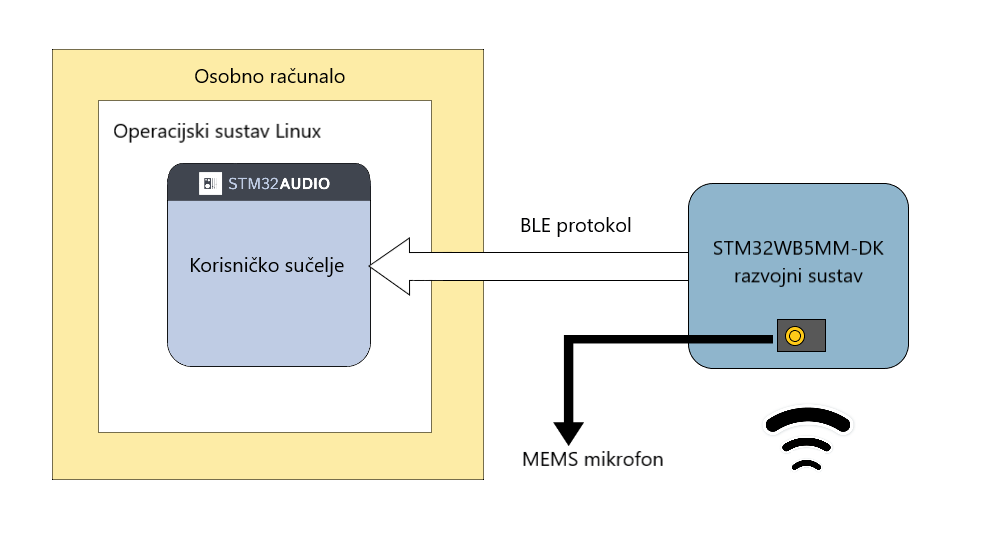
\includegraphics[width=\linewidth]{imgs/shema}
	\caption{Blok shema sustava}
	\label{fig:shema}
\end{figure}

